

\documentclass[11pt]{article}
\usepackage[margin = 1in]{geometry}
%
% ADD PACKAGES here:
%

\usepackage{amsmath,amsfonts,graphicx,amssymb}
\usepackage[backend=bibtex, sorting=none, style=numeric-comp, defernumbers]{biblatex}

\addbibresource{refs.bib}
\usepackage{tikz}
\usetikzlibrary{arrows}
\usepackage{changepage}
\usepackage{braket}
\usepackage{mathtools}
\usepackage{cite}
\usepackage{qcircuit}
\usetikzlibrary{arrows.meta}
\usepackage{tikz}
\usetikzlibrary{automata, positioning}
%
% The following commands set up the lecnum (lecture number)
% counter and make various numbering schemes work relative
% to the lecture number.
%
\newcounter{lecnum}
\renewcommand{\thepage}{\thelecnum-\arabic{page}}
\renewcommand{\thesection}{\thelecnum.\arabic{section}}
\renewcommand{\theequation}{\thelecnum.\arabic{equation}}
\renewcommand{\thefigure}{\thelecnum.\arabic{figure}}
\renewcommand{\thetable}{\thelecnum.\arabic{table}}

%
% The following macro is used to generate the header.
%
\newcommand{\lecture}[4]{
   \pagestyle{myheadings}
   \thispagestyle{plain}
   \newpage
   \setcounter{lecnum}{#1}
   \setcounter{page}{1}
   \noindent
   \begin{center}
   \framebox{
      \vbox{\vspace{2mm}
    \hbox to 6.28in { {\bf CS 4510
		\hfill } }
       \vspace{4mm}
       \hbox to 6.28in { {\Large \hfill Chomsky Hierarchy: Regular Grammars\hfill} }
       \vspace{2mm}
       \hbox to 6.28in { {\it Name: #3 \hfill} }
      \vspace{2mm}}
   }
   \end{center}
   %\markboth{Lecture #1: #2}{Lecture #1: #2}

   \vspace*{4mm}
}
%
% Convention for citations is authors' initials followed by the year.
% For example, to cite a paper by Leighton and Maggs you would type
% \cite{LM89}, and to cite a paper by Strassen you would type \cite{S69}.
% (To avoid bibliography problems, for now we redefine the \cite command.)
% Also commands that create a suitable format for the reference list.
\renewcommand{\cite}[1]{[#1]}
\def\beginrefs{\begin{list}%
        {[\arabic{equation}]}{\usecounter{equation}
         \setlength{\leftmargin}{2.0truecm}\setlength{\labelsep}{0.4truecm}%
         \setlength{\labelwidth}{1.6truecm}}}
\def\endrefs{\end{list}}
\def\bibentry#1{\item[\hbox{[#1]}]}

%Use this command for a figure; it puts a figure in wherever you want it.
%usage: \fig{NUMBER}{SPACE-IN-INCHES}{CAPTION}
\newcommand{\fig}[3]{
			\vspace{#2}
			\begin{center}
			Figure \thelecnum.#1:~#3
			\end{center}
	}
% Use these for theorems, lemmas, proofs, etc.
\newtheorem{theorem}{Theorem}[lecnum]
\newtheorem{lemma}[theorem]{Lemma}
\newtheorem{proposition}[theorem]{Proposition}
\newtheorem{claim}[theorem]{Claim}
\newtheorem{corollary}[theorem]{Corollary}
\newtheorem{definition}[theorem]{Definition}
\newenvironment{proof}{{\bf Proof:}}{\hfill\rule{2mm}{2mm}}

% **** IF YOU WANT TO DEFINE ADDITIONAL MACROS FOR YOURSELF, PUT THEM HERE:

\newcommand\E{\mathbb{E}}

\begin{document}
%FILL IN THE RIGHT INFO.
%\lecture{**LECTURE-NUMBER**}{**DATE**}{**LECTURER**}{**SCRIBE**}
\lecture{1}{}{Abrahim Ladha, John Hill}{scribe-name}
%\footnotetext{These notes are partially based on those of Nigel Mansell.}
\section{Properties}
We said every regular language is context free. Any context free language can be decided by a pushdown automata. You can convert any finite automata to a pushdown automata by simply ignoring the stack. The context free languages are also characterized by context free grammars, so it follows that there should be a class of grammars which enumerate regular languages. 

\section{Regular Grammars}
\begin{definition}
A right-regular grammar is a tuple $(V,\Sigma, P , S)$ such that:
\begin{itemize}
    \item $V$ is a set of nonterminals, sometimes called variables. These are always denoted by upper case letters
    \item $\Sigma$ is the finite alphabet, denoted by lower case letters.
    \item $P$ is a set of production rules, only of the form:
    \begin{itemize}
        \item $A \rightarrow aB$
        \item $A \rightarrow a$
        \item $A \rightarrow \epsilon$
    \end{itemize}
    \item $S \in V$ is the starting symbol.
\end{itemize}
\end{definition}
\begin{theorem}
A language is regular if and only if there exists a regular grammar to generate it.
\end{theorem}
First we show for every right-regular\footnote{left-regular grammars correspond to the reverse of the languages. It has rules of the form $A \rightarrow Aa$. This is not something we care about so much. The expressive power of regular languages, and their corresponding machines are invariant to this choice. We choose right-regular because of pedagogy.} grammar, there exists an equivalent NFA for the same language.

Given a regular grammar $G = (V,\Sigma, P , S)$, we construct an NFA $N = (\Sigma, Q, q_0, \delta, F)$
\begin{itemize}
    \item $\Sigma$ is the same
    \item $Q$ is a set of states, one for each non-terminal, plus an additional state. $Q = V \cup \{A\}$
    \item Recall that for an NFA, $\delta(\cdot, \cdot)$ is a set. For each nonterminal $B$ and character $a$:
    \begin{itemize}
        \item For each nonterminal $C$, if $B \rightarrow aC$, then $C \in \delta(B,a)$
        \item If $B \rightarrow a$, then $A \in \delta(B,a)$
        \item For each $a \in \Sigma$, define $\delta(A,a) = \emptyset$
        \item If $B \rightarrow \epsilon$, $A \in \delta(S, \epsilon)$
    \end{itemize}
    \item $q_0$, the start state is associated with the starting nonterminal, $S$. 
    \item $F = \{A\}$. 
\end{itemize}
We show $L(N) = L(G)$ by set containment
\begin{itemize}
    \item[$(L(G) \subseteq L(N))$] Let $x = a_1a_2...a_n \in L(G)$. Then there exists a production of $x$ of the form \begin{align}
        S \implies a_1A_1 \implies a_1a_2A_2 \implies ... \implies a_1a_2...a_{n-1}A_{n-1} \implies x
    \end{align} As defined, it is clear $A_1 \in \delta(S,a_1)$, and $A_i \in \delta(A_{i-1},a_i)$. It follows then that $A \in \delta(S,x)$, and $A \in F \implies x \in L(N)$. 
    \item[$(L(N) \subseteq L(G))$] Let $x \in L(N)$. If $x = \varepsilon$, then we must have that $A \in \delta(S, \varepsilon)$, but by construction this implies that $S \rightarrow \varepsilon$ is a rule of $G$. So suppose $x \neq \varepsilon$. Then there exists a sequence of states, $S, A_1, ..., A_{n-1}, A$ such that $A_1 \in \delta(S, a_1)$, and $A_i \in \delta(A_{i-1},a_i)$. This implies that we must have production rules of the form \begin{align}
        S \implies a_1A_1 \implies a_1a_2A_2 \implies ... \implies a_1a_2...a_{n-1}A_{n-1} \implies x
    \end{align} So $G$ derives $x$ and $x \in L(G)$. 
\end{itemize}
Now we show for every NFA, there exists an equivalent right-regular grammar. Let $D = (Q, \Sigma, \delta, q_0, F)$ be a DFA\footnote{Not NFA, simply because the proof is easier. It doesn't matter, because you know DFAs and NFAs have the same expressive power. } We construct a grammar $G = (V, \Sigma, P , S)$
\begin{itemize}
    \item Let $V$ correspond to the states of $Q$
    \item $\Sigma$ is the same
    \item For each rule of the form $\delta(B,a) = C$, construct a production rule of the form $B \rightarrow aC$. If $\delta(B,a) = C$, and $C \in F$, then $B \rightarrow a$. If $q_0 \in F$, then add the production rule $S \rightarrow \varepsilon$
    \item $S$ corresponds to the start state, $q_0$. 
\end{itemize} The proof is left as exercise. 
\section{Problems}
\begin{enumerate}
    \item It is true, that a regular grammar will always generate a regular language, and for each regular language, there exists a regular grammar to produce it.  But can a regular language be generated by a context free grammar which is not a regular grammar? If yes, give an example. If no, prove it. 

      \textbf{Answer.} Consider the following example, 
      \begin{align*}
        S &\to aBa \\
        B &\to b
      \end{align*}

      Clearly this generates only $aba$ and is trivially regular as it's finite. So for instance any context free grammar that is finite generates a regular language.

      \vspace{1em}
      
      Another example is to consider the language $a^{m}b^{n}$ where $m, n \in N$. Here we have the grammar, 
      \begin{align*}
        S &\to AB\\
        A &\to Aa \mid a \\
        B &\to Bb \mid b
      \end{align*}

      This is a non-regular context free grammar that produces a regular language



    \item We constructed a grammar $G$ given an NFA $M$. Prove that $S \stackrel{*}{\implies} x \iff \delta(q_0,x) \in F$. Just follow the reverse of the proof we showed.


      \textbf{Answer. } So first we have $S \stackrel{*}{\implies} x$, we need to show this implies that $\delta(q_{0}, x) \in F$. Clearly if $S \stackrel{*}{\implies} x$ then if $x = a_{1} \dots a_n$ then we have a series of productions of $x$ of the form $S \implies a_{1}A_{1} \implies a_{1}a_{2} \dots a_{n - 1}A_{n - 1} \implies x$. Now as $S$ corresponds to the start state $q_{0}$ and for each non-terminal we have $q_{i}$ corresponding to $A_i$ (for $i \in \{1, \dots, n - 1\}$) note that if we traverse the string $a_{1}, \dots, a_{n}$ we have $q_i \in \delta(q_{i - 1}, a_i)$ and if $A_{n - 1} \to a_n$ then we know have by definition $q_n \in \delta(q_{n -1}, a_n)$ (for simplicity we have $q_n = A$ instead i.e our accept state) so we have, 
      \[
        q_n \in  \delta(\dots \delta(\delta(q_{0}, a_{1}), a_{2}), a_n) = \delta(q_{0}, x)
      \]

      and we have $q_n \in F$ by definition  so we get $\delta(q_0, x) \in F$

      \vspace{1em}
      
      Now looking at the reverse we have $\delta(q_{0}, x) \in F$ and we need to show that $S \stackrel{*}{\implies} x$. Now if $\delta(q_{0}, x) \in F$ then we have a sequence of state $q_{0}, \dots, q_n$ such that $q_n \in F$ and $\delta(q_{i - 1}, a_i) = q_i$. Now clearly as $q_{0}$ corresponds at $S$ and we as each state $q_i$ other than the accept and start state will correspond to some arbitrary non-terminal state say $B_i$ we have if $q_i \in \delta(q_{i -1 }, a_i)$ this implies that $B_{i - 1} \to a_i B_{q_i}$ so putting it all together if we have $\delta(q_0, x) = q_n \in F$ then this means we have, 
      \[
        \delta(q_{0}, x) = \delta(\dots \delta(\delta(q_{0}, a_{1}), a_{2}), a_n)\in F
      \]

      which means that we get, 
      \[
        S \implies a_{1}A_{1} \implies a_{1}a_{2} \dots a_{n - 1}A_{n - 1} \implies x
      \]

      or $S \stackrel{*}{\implies} x$




    \item Consider the regular language $\{x \in \Sigma^* ~|~ x \text{ has an even number of 0s}\}$. Give the minimal DFA for this language, and construct the right-regular grammar for that DFA (following the construction in the proof). 

      \textbf{Answer.} The minimal DFA is as follows,
      \begin{center}
      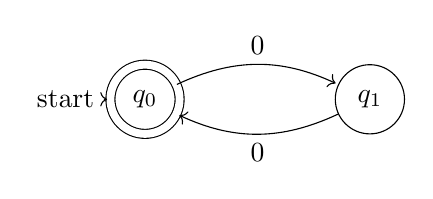
\begin{tikzpicture}[shorten >=1pt,node distance=2cm,on grid,auto,scale=0.17]
      \tikzset{accepting/.style={double distance=1mm}}
      \node[state,initial,accepting, label=center:{$q_0$}] (0) at (23.3,-29.4) {};
      \node[state, label=center:{$q_1$}] (1) at (40.1,-29.4) {};
      \path[->] (0) edge[bend left=25 ] node {$0$} (1);
      \path[->] (1) edge[bend left=25 ] node {$0$} (0);
      \end{tikzpicture}
      \end{center}

      Now in order to construct the right regular language first we have $V = Q = \{q_{0}, q_{1}\}$ which  is our set of non-terminals, let $S =_{0}$ and $A = q_{1}$. Now we're assuming our alphabet is $\Sigma = \{0\}$ so we have two rules $\delta(q_{0}, 0) = q_{1}$ and $\delta(q_{1}, 0) = q_{0}$ which corresponds to the rules $S \to 0A$ and $A \to 0S$. And as we have $\delta(q_{1}, 0) = q_{0}$ and $q_{0} \in F$ we have $q_{1} = A \to 0$. And as $q_{0} \in F$ we have $S \to \epsilon$. Putting this together we get, 
      \begin{align*}
        S &\to 0A \mid \epsilon\\
        A &\to 0S \mid 0\\
      \end{align*}


      \vspace{1em}
      
      (If we assume we have other alphabets as well then in our DFA we just have all the symbols at $q_{0}$ and $q_{1}$ except $0$ go to itself which just corresponds $\delta(q_{1}, a) = q_{1}$  which is the production $A\to a A$ for $a \ne 0$ and $\delta(q_{0}, a) = q_{0}$ which is $S \to aS$ for $a \ne 0$ and as $S$ is the end state we also have $S \to a$ for $a \ne 0$)

    \item For the language $\{0^i1^j ~|~ i, j \geq 0\}$ give the minimal\footnote{We haven't talked about what a minimal regular grammar is, so just give the smallest (with respect to number of nonterminals) one you can come up with} right-regular grammar for this language, then construct the NFA associated with that grammar. 

      \textbf{Answer. } The minimal right regular grammar is, 
      \begin{align*}
        S &\to 0S \mid B \mid \epsilon\\
        B &\to 1B \mid \epsilon
      \end{align*}

      Now to convert it into an NFA we have,
\begin{center}
  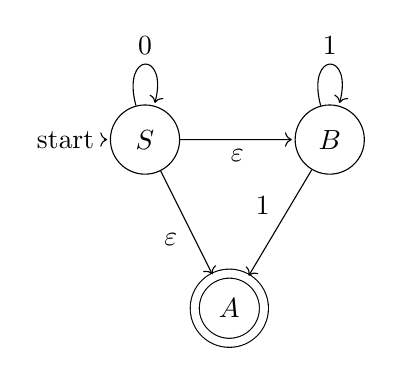
\begin{tikzpicture}[shorten >=1pt,node distance=2cm,on grid,auto,scale=0.17]
\tikzset{accepting/.style={double distance=1mm}}
\node[state,initial, label=center:{$S$}] (0) at (25.8,-24.6) {};
\node[state, label=center:{$B$}] (1) at (39.6,-24.6) {};
\node[state,accepting, label=center:{$A$}] (2) at (32.1,-37.2) {};
\path[->] (0) edge node [swap] {$\varepsilon$} (1);
\path[->] (1) edge node [swap] {$1$} (2);
\path[->] (0) edge[loop above] node {$0$} ();
\path[->] (1) edge[loop above] node {$1$} ();
\path[->] (0) edge node [swap] {$\varepsilon$} (2);
\end{tikzpicture}
\end{center}

    \item Let $A_1,A_2$ be any non terminals and let $a_1,...,a_n$ be any terminals. Prove that a production rule of the form $A_1 \rightarrow a_1...a_nA_2$ can be converted to a set of production rules of a regular grammar. 

      \textbf{Answer. } What we need to show that there is an equivalent regular grammar to the above. We do this by introducing new non-terminals. Let, 
      \[
        B_1 \to a_{2} \dots a_n A_{2}
      \]
      then we have, 
      \begin{align*}
        A_{1} &\to a_{1} B_{1}
      \end{align*}

      Now this leaves us with a non regular grammar for $B_{1}$ which is, 
      \[
        B_{1} \to a_{2} \dots a_n A_{2}
      \]

      but note that we have one less terminal in the left side. So inductively we do this $n - 1$ times until we have, 
      \[
        B_{n - 1} \to a_n A_{2}
      \]

      So now we have the group of productions, 
      \begin{align*}
        A_{1} &\to a_{1}B_{1} \\
        B_{1} &\to a_{2} B_{2}\\
              &\dots\\
        B_{n - 2} &\to a_{n - 1}B_{n - 1}\\
        B_{n - 1} &\to a_n A_{2}
      \end{align*}

      Now note that each of this productions correspond to a regular grammar. So we're done.
\end{enumerate}
\nocite{*}
\printbibliography[title={Further Reading},notcategory=cited]
\end{document}
